\documentclass[11pt]{article}
\usepackage{fullpage}
\usepackage{amsmath, multirow}
\usepackage{amssymb}
\usepackage{amsthm}
\usepackage{xcolor}
\usepackage{hyperref}
\usepackage{graphicx}

\newcommand{\dist}{\mathrm{\bf dist}}
\pagestyle{empty}

%\parskip .125in

\begin{document}
\begin{center}
{\bf Intro to Computational Math, Fall 2025\\
Section 2, Sept 5 (not due or graded).\\
}
\end{center}

\noindent {\it Section will give you time to work on/discuss questions in small groups and then present your solutions. The questions below are selected exercises from the textbook to help build comfort and expertise with the ideas we've been discussing. The last question is from a prior exam in this course.
\\
}

\noindent {\bf Q1.} Attempt Exercise 3 in Section 2.1 and Exercises 2 and 3 of Section 2.3 of Driscoll and Braun (\url{https://fncbook.com/}).

\vskip1cm

\noindent {\bf Q2.}  Consider the functions $f,g\colon \mathbb{R}\rightarrow\mathbb{R}$: \footnote{Here $\log(t)$ denotes the natural logarithm of $t$ and $\exp(t)$ denotes $e^t$ with $e=2.7182\dots$.}
$$ \begin{cases} 
f(x) &= \log(\exp(x) + \exp(-x)) \\
g(x) &= \log(1 + \exp(-2|x|)) + |x| \ . 
\end{cases} $$
These two functions are actually equal (that is, for all $x\in\mathbb{R}$ $f(x)=g(x)$)!\\ Despite this, the implementations below evaluate to different values at $x=1234.56789$.\\
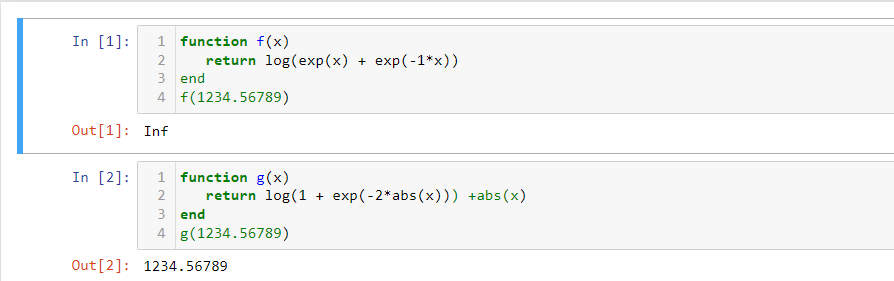
\includegraphics[width=\textwidth]{logSumExp.png}
\begin{description}    
    \item[(a)] What is the condition number of $f$ at $x=1234.56789$?\\
    (A formula with several log() and exp() is fine, don't worry about simplifying beyond that.)\\

    \vskip0.7cm

    \item[(b)] Explain why a computer using standard IEEE floating point arithmetic will fail to compute $f(1234.56789)$ properly. As seen above, a direct implementation produced \texttt{Inf} instead of a numerical answer {\it (Hint: Based on (a), the problem here is not bad conditioning)}.\\

    \vskip0.7cm

    \item[(c)] Based on (a), provide an approximate upper bound on the error in the above from evaluating $g$ using standard IEEE floating point arithmetic. Namely, state a number $U$ with $$ |g(1234.56789) - 1234.56789| \leq U \ .$$
    (A formula with several log() and exp() is fine, don't worry about simplifying beyond that.)
\end{description}


\end{document} 